% Chapter Template

\chapter{Marco Teórico} % Main chapter title

\label{Chapter2} % Change X to a consecutive number; for referencing this chapter elsewhere, use \ref{ChapterX}

%----------------------------------------------------------------------------------------
%	SECTION 1
%----------------------------------------------------------------------------------------

\section{Contexto}

Una de las líneas de desarrollo de BQ es la robótica educativa, un conjunto de productos y servicios orientados a educar en las tres partes de todo proyecto tecnológico: Diseño, hardware y software. Cuenta para ello con diferentes productos (impresoras -Witbox, hephestos-, "mi primer kit de robótica", o los printbots), programas (Bitbloq -basado en scratch-), así como contenido y soporte en la web ("Do it with others" -www.diwo.bq.com-).

El presente proyecto surge de la necesidad de automatizar una parte del proceso de fabricación de un nuevo robot educativo, Zowi. Hasta ahora, los robots desarrollados (printbots, por su carácter de chasis y componentes no-electrónicos totalmente imprimibles en 3d) usaban para moverse servos de rotación continua y ruedas, Zowi es el primer robot bípedo desarrollado por BQ (utiliza dos servos de posición para los piés y otros dos para las caderas) y la librería de osciladores sinusoidales -Oscillator-, desarrollada por Juan "Obijuan" González, entonces jefe del departamento, para robots serpiente modulares.

\subsection{Zowi}
Zowi, también llamado el robot de Clan TVE, es un robot educativo para niños que les inicia en el mundo de la tecnología y de la programación. Se puede ver el juguete en la Figura \ref{fig:Zowi-img}.

\begin{figure}[h]
\centering
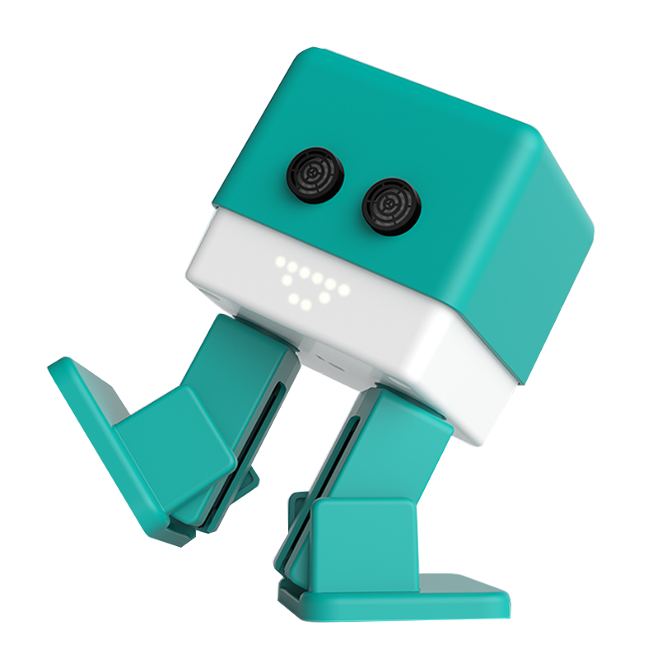
\includegraphics[width=110mm]{Figures/zowi-img.png}
\caption[Robot Zowi]{Robot Zowi}
\label{fig:Zowi-img}
\end{figure}

Este robot, movido por una controladora basada en Arduino y diseñada a medida para él, además de los servos que lo convierten en un robot bípedo, incorpora unos sensores de ultrasonidos como ojos que le permiten detectar obstáculos, una matriz de leds como boca para expresar "emociones" y tres pequeños botones para alternar entre sus modos de funcionamiento, entre otros componentes.

Se ha creado una aplicación móvil, Zowi App, que permite controlar los movimientos de Zowi y reprogramarlo fácilmente con diferentes juegos. Zowi tiene muchas posibilidades más allá de lo predefinido en su aplicación. BQ tiene una plataforma online para programar a sus robots y controladoras, esta plataforma se llama Bitbloq. En Bitbloq se puede programar a Zowi y a otros tipos de placas Arduino de forma muy sencilla por medio de bloques, sin necesidad de saber ningún lenguaje de porgramación. La opción de emplear código directamente tambien está disponible.

\section{Motivo del proyecto}
La tarea asignada al autor del proyecto fue la de idear y desarrollar el prototipo de \textbf{un sistema capaz de ajustar de forma automática cada uno de los cuatro servos que componen las piernas de Zowi}, lo que permite al robot ejecutar sus programas de fábrica, con los que saldrá a la venta, de forma correcta; entre ellos: realizar diferentes bailes, caminar, etc. Dicho sistema debe ser utilizado por operaradores sin conocimientos de Arduino ni de electrónica en general. La nacionalidad de los operarios tambien es desconocida por no saberse el emplazamiento de la fábrica hasta más avanzado el proyecto (razón por la que parte de la documentación anexada se encuentra en inglés: menú de la interfaz, comentarios del código, etc).

\subsection{Servos}
Los servos son un tipo especial de motor DC que se caracterizan por su capacidad para posicionarse de forma inmediata en cualquier posición dentro de su intervalo de operación. Para ello, el servomotor espera un tren de pulsos que se corresponde con el movimiento a realizar. Están generalmente formados por el motor, un sistema reductor formado por ruedas dentadas, un potenciómetro y un circuito de realimentación, todo en un misma caja de pequeñas dimensiones. En la Figura \ref{fig:futaba}, se muestra un servomotor del tipo empleado en Zowi.

\begin{figure}[h]
\centering
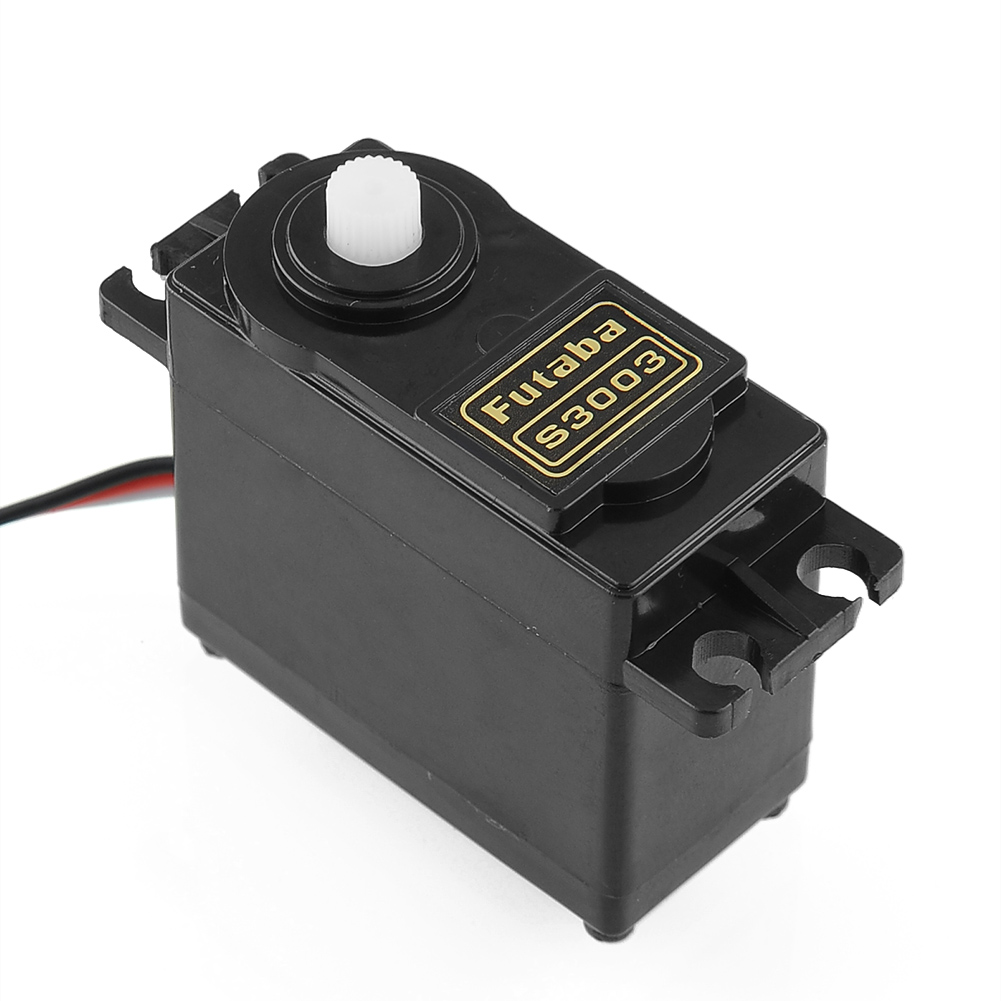
\includegraphics[width=90mm]{Figures/futaba.png}
\caption[Servo Futaba S3003]{Servo Futaba S3003}
\label{fig:futaba}
\end{figure}

El circuito electrónico de realimentación del servo es el encargado de recibir la señal PWM y traducirla en movimiento del Motor DC. El eje del motor DC está acoplado a un potenciómetro, el cual permite formar un divisor de voltaje. El voltaje en la salida del divisor varía en función de la posición del eje del motor DC. En la Figura \ref{fig:ServoDiag} se muestra un diagrama del funcionamiento de un servo de posición.

\begin{figure}[h]
\centering
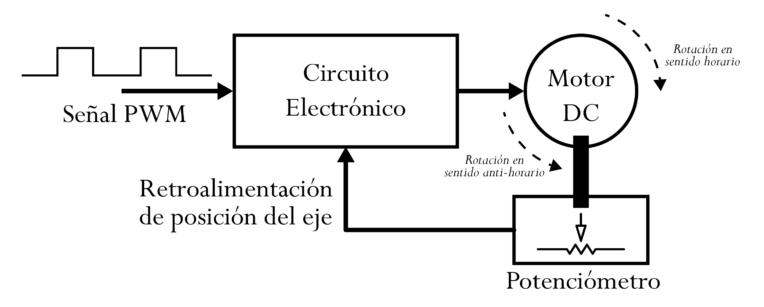
\includegraphics[width=140mm]{Figures/servo-diag.png}
\caption[Diagrama de bloques servomotor]{Diagrama de bloques servomotor}
\label{fig:ServoDiag}
\end{figure}


La modulación por anchura de pulso, PWM (Pulse Width Modulation), es una de los sistemas más empleados para el control de servos. Este sistema consiste en generar una onda cuadrada en la que se varía el tiempo que el pulso está a nivel alto, manteniendo el mismo período, con el objetivo de modificar la posición del servo según se desee. Arduino permite generar PWM en algunos de sus pines de forma sencilla, además, para hacerlo aún más fácil, tiene la librería \textit{srvo.h}, que nos permite dar un valor de posición angular (grados) a un determinado pin, y él sólo genera el PWM.

Las señales de PWM requeridas por el circuito de control electrónico son similares para la mayoría de los modelos de servo. Esta señal tiene la forma de una onda cuadrada. Dependiendo del ancho del pulso, el motor adoptará una posición fija. Un ejemplo visual en la Figura \ref{fig:ServoPWM}.

\begin{figure}[h]
\centering
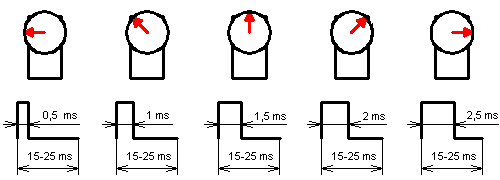
\includegraphics[width=140mm]{Figures/servo-pwm.png}
\caption[Posición según PWM]{Posición según PWM}
\label{fig:ServoPWM}
\end{figure}

\subsection{Problema a resolver}
Los servos empleados son una versión clónica del Futaba S3003 que vimos en la Figura \ref{fig:futaba}, con un rango de funcionamiento algo mayor (en torno a 193º). Para el caso de Zowi, el rango empleado será bastante menor, por cuestiones de estabilidad del juguete y por el diseño de las piezas, mecánicamente sería imposible torcer las articulaciones en todo el rango del servomotor.

La continuación del eje del servo, eje dentado, engrana en la pieza de Zowi. Como podemos ver en la Figura \ref{fig:EjeServo} a modo ilustrativo, hay un determinado número de dientes en dicho engranaje; para el servo empleado en Zowi, hay 24 dientes en el engranaje, por lo que un diente supone un cambio de 15º respecto al anterior.

\begin{figure}
\centering
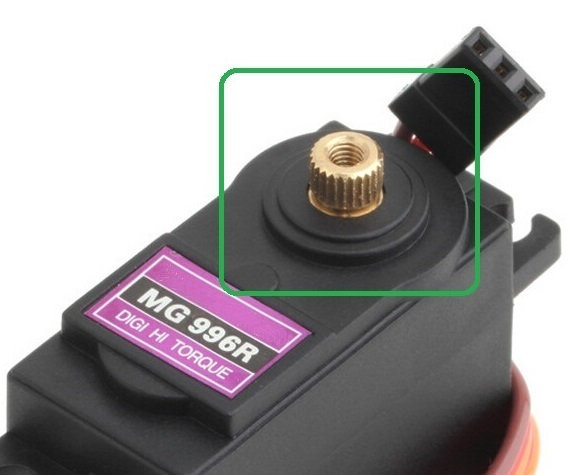
\includegraphics[width=80mm]{Figures/servo-shft.jpg}
\caption[Eje dentado servo]{Eje dentado servo}
\label{fig:EjeServo}
\end{figure}

El ensamblaje de los servos en sus piezas correspondientes se hace de forma manual, se hace que el servo llegue a hacer tope en uno de los sentidos como referencia y es engranado de forma que tenga disponible el rango de funcionamiento necesario. Sin embargo, dentro de los 15º que se comentaban anteriormente, y por la misma fabricación de las partes del servo, las piezas podrían quedar montadas con un desfase de hasta 7.5 grados, o mayor aún si el operador no elige bien la orientación al engranar. Adicionalmente, por el fabricante del servo, la relación entre tren de pulsos PWM y la posición final del servo puede variar -estar un poco desplazada-, incluso variar muy ligeramente entre servos del mismo fabricante.

Se tienen entonces varios factores que hacen que cada servo sea montado en una posición distinta -o considerada distinta por el programa- y tenga que ser configurado por software, además, el ajuste se adaptará para cada servo, no se puede definir una regla válida para todos, de ahí que se emplee un método iterativo para solucionarlo.

Lo ideal sería que la posición del servo intermedia coincidiese con la posición neutra de la articulación de Zowi, dejando la mitad del rango de giro del servomotor para cada sentido. Sin embargo, como el rango de movimiento del juguete es menor que el rango completo del servo, se tiene un margen bastante generoso que se puede corregir en el ajuste.

\subsubsection{Calibración}
La calibración de los servos es de importancia vital para un buen funcionamiento de las funciones programadas en el juguete y en cualquier aplicación que utilice servos, en general. En Arduino, utilizando la librería \textit{srvo.h}, se consiguen generar los pulsos PWM de forma transparente, empleando directamente grados sexagesimales (números enteros). El primer paso para utilizar un servo es siempre definir qué posición es la de partida del servo, es decir, fijarle un 0º. Ésto se realiza guardando un valor ("trim" u "offset") que podrá ser positivo o negativo y se empleará para corregir las orientaciones.

Cuando el usuario quiere mover el servo a una posición determinada utilizando la librería \textit{srvo.h} directamente, tendrá que moverlo a la posición deseada más el valor de "offset". El offset obviamente siempre será el mismo para cada servo, salvo que se desmonte y monte el servo en otra posición o en otra pieza y se tenga que recalibrar. Este ajuste es habitual cuando se trabaja con servos, en robótica o radiocontrol por ejemplo.

Sabemos que Zowi es un producto pensado para ser reprogramado y "trasteado", para que el usuario aprenda sobre electrónica y programación; sin embargo, éste usuario no tiene por qué tener ningún conocimiento previo en el momento de adquirir el robot, es por ésto que Zowi sale a la venta con programas por defecto, programas que muestran sus posibilidades. Zowi tendrá los valores de "offset" de los servos, calculados para su montaje en fábrica, guardados en determinadas direcciones de la EEPROM, zona de la memoria de la placa controladora que no se borra al ser reprogramada por el usuario.

\section{Posibles alternativas}

Anteriormente, se ha explicado cuál es el problema a resolver. Para darle solución, la clave es poder leer las orientaciones reales de los servos, es decir, las orientaciones respecto al mismo juguete; en base a estas posiciones se debe actuar sobre los servos hasta colocarlos en la posición neutra y guardar en la memoria el desfase observado para cada servo. Se plantean dos posibles caminos:

\begin{itemize}
  \item \textbf{Visión por computador:} Emplear un sistema de visión para, mediante matching y detección de líneas, observar el desvío y poder actuar sobre los servomotores hasta llevarlos a la posición deseada.
  \item \textbf{Sensor IMU:} Utilizar utillaje impreso y sensores de tipo inercial (acelerómetro-giróscopo) para calcular las inclinaciones producidas por la posición de los servos.
\end{itemize}

Se elige la segunda opción por tener una estimación de tiempo de desarrollo más ajustada, además de un coste considerablemente menor.

\subsection{Sensor IMU}
Se describe brevemente la utilidad del sensor IMU ya que todo el sistema se construye en torno a este componente.

Una IMU, o unidad de medición inercial, es un sensor diseñado para combinar las características de un acelerómetro y un giróscopo, y mostrar información completa sobre aceleración, posición, orientación, velocidad...

Las medidas crudas de los componentes del acelerómetro, giróscopo y magnetómetro (encapsulado junto al acelerómetro) estarán directamente relacionadas con la fuerza G, velocidad angular y campo magnético, respectivamente. Dichas medidas pueden ser procesadas y tratadas con un microcontrolador o microprocesador para obtener posiciones, orientaciones, etc.

\subsubsection{Acelerómetro}

El acelerómetro mide la aceleración en las 3 dimensiones del espacio. La gravedad de la Tierra tiene una aceleración perpendicular al suelo. Así pues, la IMU también detecta la aceleración de la gravedad terrestre. Gracias a ésta se pueden usar las lecturas del acelerómetro para saber cuál es el ángulo de inclinación respecto al eje X o eje Y. Figura \ref{fig:ImuAcel}.

\begin{figure}[h]
\centering
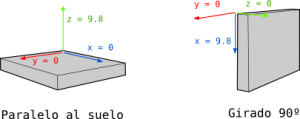
\includegraphics[width=90mm]{Figures/imu-acel.png}
\caption[Lectura acelerómetro]{Lectura acelerómetro}
\label{fig:ImuAcel}
\end{figure}

Dado que el ángulo se calcula a partir de la gravedad, no es posible calcular el ángulo Z empleando únicamente el acelerómetro. Para hacerlo se necesita otro componente: el magnetómetro, que es simplemente un tipo de brújula digital.

\subsubsection{Giróscopo}

El giróscopo es un dispositivo que mide la velocidad angular en cada uno de los ejes. Figura \ref{fig:ImuGiro}.

\begin{figure}[h]
\centering
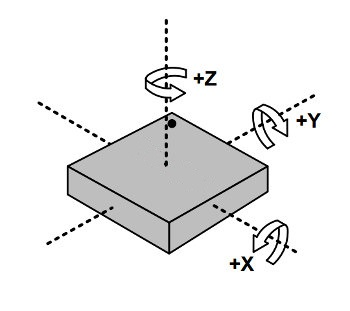
\includegraphics[width=60mm]{Figures/imus-giro.jpg}
\caption[Lectura giróscopo]{Lectura giróscopo}
\label{fig:ImuGiro}
\end{figure}

%-----------------------------------
%	SUBSECTION 1
%-----------------------------------
\section{Herramientas y tecnologías utilizadas}

Además de los componentes electrónicos que se han introducido anteriormente y los que se tratarán en el capítulo de desarrollo: Capítulo \ref{Chapter3}, cabe mencionar las tecnologías y herramientas que han resultado útiles durante todo el proyecto.

\subsection{Máquinas}

La tecnología de impresión 3D por FFF ha aportado agilidad al proyecto al permitir la creación de piezas en el mismo lugar en cuestión de horas. Se han empleado máquinas \textbf{Hephestos} (Figura \ref{fig:hephestos}) y \textbf{Witbox} (Figura \ref{fig:witbox}) de BQ, ambas con firmware \textbf{Marlin}, para la creación del utillaje provisional y componentes menores como los soporte de las placas dentro del armario o la caja que contiene el display LCD y el zumbador.

\begin{figure}[h]
\centering
\begin{minipage}{.52\textwidth}
  \centering
  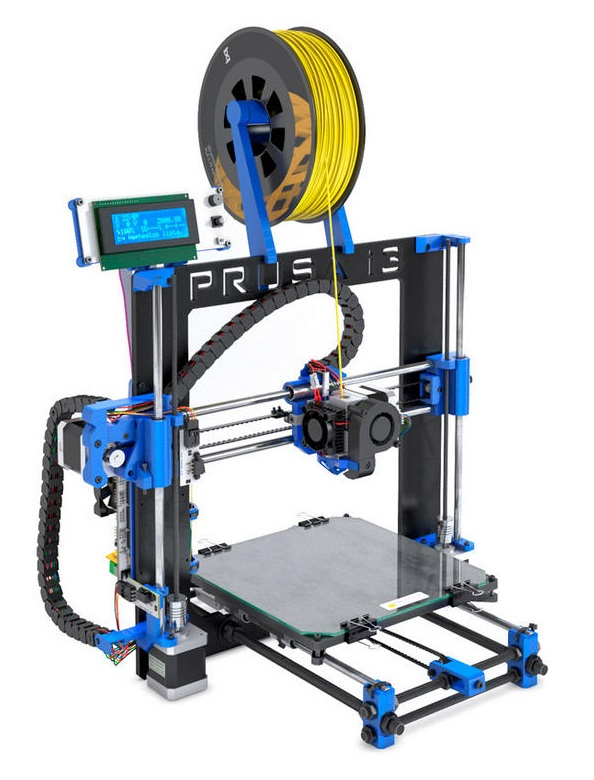
\includegraphics[width=0.9\textwidth]{Figures/hephestos}
  \captionof{figure}{Hephestos}
  \label{fig:hephestos}
\end{minipage}%
\begin{minipage}{.48\textwidth}
  \centering
  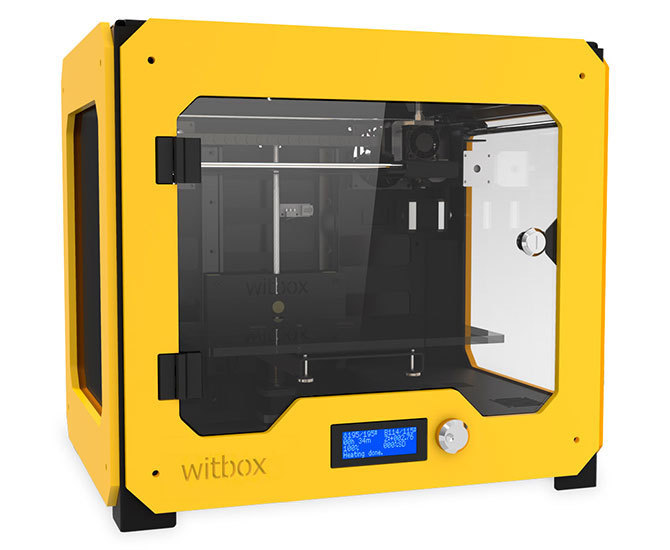
\includegraphics[width=1\textwidth]{Figures/witbox}
  \captionof{figure}{Witbox}
  \label{fig:witbox}
\end{minipage}
\end{figure}

Otra máquina interesante fue la fresadora \textbf{Cyclone} (Figura \ref{fig:cyclone}), entonces en fase beta. Se montó y empleó para el primer prototipo de la PCB de la shield desarrollada.

\begin{figure}[h]
\centering
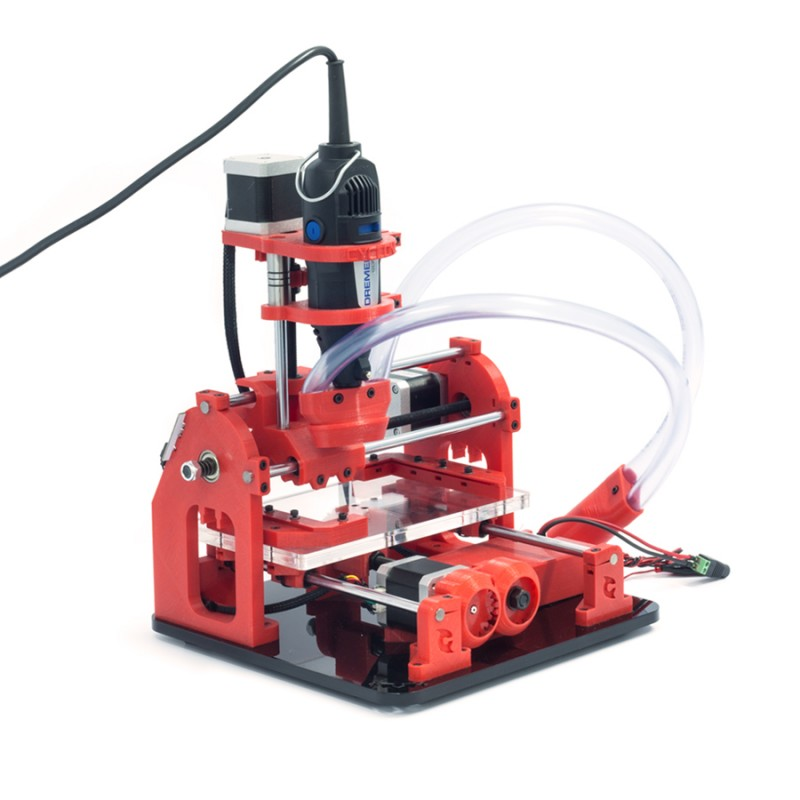
\includegraphics[width=90mm]{Figures/cyclone.jpg}
\caption[Cyclone]{Cyclone}
\label{fig:cyclone}
\end{figure}

\subsection{Diseño}

Para el diseño de las piezas impresas se ha utilizado \textbf{Inventor} y \textbf{FreeCad}, el laminado se ha llevado a cabo con \textbf{Cura}.

El diseño de la PCB y la generación de los gerbers se logró mediante \textbf{KiCad}. Su fresado fue posible gracias a \textbf{FlatCAM} y \textbf{CNCGcodeController}.

Los planos eléctricos se han creado con \textbf{DraftSight}.

\subsection{Programación}

El desarrollo de los programas de Arduino y la programación de las controladoras se ha llevado a cabo empleando el mismo IDE de Arduino clásico: \textbf{Arduino 1.0.6}.

El sistema operativo instalado en Raspberry ha sido la versión adaptada de Debian: \textbf{Raspbian}, la versión concreta, última a la fecha: Raspbian Wheezy.

El programa principal de la Raspberry ha sido desarrollado en \textbf{Python 2.7.11}, última versión de Python 2 a la fecha. Ha sido útil el editor \textbf{Atom} y su capacidad de acceder a los directorios remotos directamente, mediante SFTP.

\subsection{Post-desarrollo}

Para acceso remoto, troubleshooting y extracción de los datos se han utilizado las siguientes herramientas:
\begin{itemize}
  \item \textbf{Putty} para las conexiones SSH.
  \item \textbf{Filezilla} y \textbf{WinSCP} para acceso remoto a ficheros.
  \item \textbf{HeidiSQL} para acceso a la base de datos.
\end{itemize}

La documentación del proyecto se ha realizado en \textbf{\LaTeX} con \textbf{Atom} y \textbf{TeXworks}.
